\subsection{Notfall-Evakuierung mit einem Service-Roboter}
\label{subsec:evacuation}
    Mit dem Szenario der Notfall-Evakuierung wird ein weiterer Anwendungsfall definiert, der die 
    Anforderungen zu identifizieren hilft, die für die Bereitstellung des Frameworks der Steuerzentrale benötigt werden. 
    \\
    \linebreak
    Objektiv betrachtet gibt es bei diesem Fall ebenso einen Auslöser, bspw. einen Rauch- 
    oder Gasmelder, der eine \acs{MQTT}-Nachricht veröffentlicht, die über die Steuerzentrale konsumiert und verarbeitet wird. Die 
    weiteren notwendigen Schritte, die der Entwickler vorab festgelegt hat, werden von dieser Steuerzentrale eingeleitet. 
    Nachdem das \acs{MQTT}-Topic, das die entsprechende Nachricht enthält, von der Steuerzentrale empfangen wurde, wird 
    basierend auf dem Nachrichteninhalt die Regel und die darauffolgende Aktion angestoßen. Am Beispiel eines Rauchmelders 
    als Auslöser würde die Steuerzentrale über die \acs{API} 
    Schnittstelle den vorab vom Entwickler festgelegten Check des internen Büroplatzbuchungssystems durchführen, um alle 
    eingecheckten Personen und Platzbuchungen abzufragen und 
    zwischenzuspeichern. Die Informationen werden genutzt, um den Service-Roboter an die Arbeitsplätze der jeweilig 
    eingecheckten Personen zu schicken und über den Notfall zu informieren, bzw. zum Verlassen des Gebäudes aufzufordern. 
    Ist eine Person nicht an ihrem Arbeitsplatz, soll der Service-Roboter den nächsten Arbeitsplatz ansteuern. Nach Kontrolle aller 
    Arbeitsplätze soll der Service-Roboter die restliche erreichbare Bürofläche abfahren und nach Personen 
    Ausschau halten. Die Erkennung der Person wird durch die Kamera des Roboters durchgeführt. Abschließend soll der Roboter 
    an eine zentrale Stelle im Büro fahren und ohne Unterbrechung eine 
    Durchsage starten und diese solange wiederholen, bis eine Person den Vorgang manuell beendet. Mit der Beendigung der Dauerschleife 
    ist das Szenario abgeschlossen und der Roboter kann an seine Ausgangsposition zurückgeführt werden, sofern dies 
    umgebungsbedingt noch möglich ist. Die grobe Skizzierung ist folgendem Anwendungsfalldiagramm zu entnehmen: 
    \begin{figure}[hbt!]
        \centering
        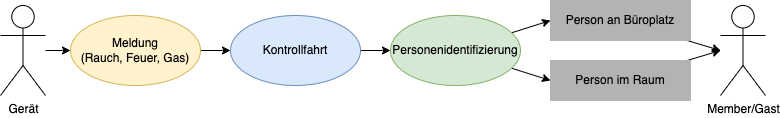
\includegraphics[width=15cm,height=15cm,keepaspectratio]{images/UC2_Diagramm_Notfall.png}
        \caption{Use Case 2 - Anwendungsfalldiagramm}
        \label{fig:uc2-emergency}
    \end{figure}
    \\
    %\linebreak
    Die Anwendungsfälle wurden so gewählt, da diese eine gewisse Komplexität mit sich bringen, die es mit der Steuerzentrale 
    abzudecken gilt.
    \\
    \linebreak
    Zur Stützung der textuellen Schilderung des zweiten Anwendungsfalls werden nachfolgend Diagramme dargestellt, die das Szenarium 
    widerspiegelt. Im Rahmen des \acs{RE} wurden hierfür ebenso eine konkrete Aufgabenbeschreibung, sowie eine User Story und ein Ablaufdiagramm definiert. Diese sind dem 
    Anhang (siehe Anhang \ref{appendix:user-story-uc2}) zu entnehmen. Die folgenden Abbildungen setzen sich aus einem 
    Aktivitätsdiagramm und einem Sequenzdiagramm zusammen: %und einem Ablaufdiagramm zusammen: 
    %\\
    %Aus dem Kontext beider Anwendungsfälle, der vorangestellten Zielgruppenanalyse und den Experteninterviews werden in Abschnitt 
    %(\ref{sec:requirementsFinal}) die daraus identifizierten Anforderungen für die Steuerzentrale aufgeführt.
    